\section{Experimental Evaluation}
\label{sec:experiments}

\subsection{Experimental Setup}
\label{sec:exp_setup}

\paragraph{Datasets and Statistical Heterogeneity.}
We conduct empirical evaluations on two vision benchmarks:
\begin{enumerate}
    \item \textbf{FEMNIST}~\cite{caldas2018leaf}: 62 fine-grained handwritten character classes ($28 \times 28$ grayscale images) with 15,000 training and 3,000 test images partitioned across $N=15$ clients.
    \item \textbf{CIFAR-100}~\cite{krizhevsky2009learning}: 60,000 $32 \times 32$ color images partitioned across $C=100$ categories with 10,000 training and 3,000 test images partitioned across $N=10$ (and scaled to $N=50$) edge clients.
\end{enumerate}
To evaluate robust personalization under progressive data skew, we partition training samples across clients using symmetric Dirichlet distributions $\mathrm{Dir}(\alpha)$ spanning five regimes: \textbf{IID} ($\alpha = \infty$), \textbf{Mild} ($\alpha = 1.0$), \textbf{Moderate} ($\alpha = 0.5$), \textbf{Severe} ($\alpha = 0.1$), and \textbf{Extreme} ($\alpha = 0.05$). Under extreme skew ($\alpha = 0.05$), each client holds samples from only 3--6 distinct classes, representing acute real-world edge non-IID conditions.

\paragraph{Baselines.}
We benchmark \fedhep{} against six prominent FL baselines spanning three major paradigms:
\begin{itemize}
    \item \textbf{Global Consensus}: \textsc{FedAvg}~\cite{mcmahan2017communication}, \textsc{FedProx}~\cite{li2020federated} ($\mu=0.01$), and \textsc{SCAFFOLD}~\cite{karimireddy2020scaffold}.
    \item \textbf{Byzantine-Robust Baseline}: \textsc{Multi-Krum}~\cite{blanchard2017machine}.
    \item \textbf{Personalized FL}: \textsc{Ditto}~\cite{li2021ditto} (dual-model bi-level regularization with proximal penalty $\lambda=0.05$) and \textsc{FedRep}~\cite{collins2021exploiting} (decoupled local heads with alternating updates).
\end{itemize}

\paragraph{Models, Budget FL Protocols, and Edge Profiling.}
For primary benchmarks, all methods employ a compact ResNet-9 backbone ($d=512$, $1.65\mathrm{M}$ parameters). For real-world edge resource profiling, we evaluate MobileNetV3-Small~\cite{howard2019searching} ($d=576$, $1.53\mathrm{M}$ parameters) utilizing depthwise separable convolutions. Under a realistic edge budget regime, communication rounds are parameterized as $R=25$ for multi-regime benchmarks, $R=30$ for Byzantine poisoning sweeps, and $R=20$ (and $R=40$) for 50-client scalability. Training utilizes local compute budget $E=3$ epochs per round, batch size $B=64$ (ResNet-9) / $B=32$ (MobileNetV3), SGD with momentum $0.9$, learning rate $\eta \in [0.02, 0.05]$, and weight decay $5 \times 10^{-4}$. All benchmark runs report mean and standard deviation across three independent random seeds ($\{42, 123, 7\}$).

\paragraph{Evaluation Metrics.}
We evaluate two principal metrics: (1) \textbf{Average Personalized Accuracy (Top-1 Acc)}, evaluated locally on each client's private test partition; and (2) \textbf{Worst-Decile Tail Fairness (Bottom 10\%)}, computed as the average test accuracy of the lowest-performing 10\% of clients.

\subsection{Multi-Scale Personalization under Extreme Heterogeneity}
\label{sec:exp_personalization}

Table~\ref{tab:main_benchmark_femnist} and Figure~\ref{fig:femnist_personalization} report personalization accuracy and bottom-10\% fairness on FEMNIST across the five Dirichlet skew regimes. In benign IID settings, global consensus models (\textsc{FedAvg}, \textsc{FedProx}, \textsc{SCAFFOLD}) achieve solid accuracy ($\approx 84\%$), but degrade steadily as skew intensifies. In contrast, \fedhep{} matches or outperforms personalized baselines across all non-IID regimes, reaching $94.73\%$ accuracy and $83.91\%$ bottom-10\% fairness under extreme skew ($\alpha=0.05$).

\begin{table*}[t]
\centering
\caption{\textbf{Personalization Benchmark across 5 Heterogeneity Regimes on FEMNIST ($C=62$, ResNet-9).} Mean $\pm$ std across 3 independent seeds. Best results in \textbf{bold}.}
\label{tab:main_benchmark_femnist}
\resizebox{\textwidth}{!}{
\begin{tabular}{lcccccccccc}
\toprule
 & \multicolumn{2}{c}{\textbf{IID ($\alpha=\infty$)}} & \multicolumn{2}{c}{\textbf{Mild ($\alpha=1.0$)}} & \multicolumn{2}{c}{\textbf{Moderate ($\alpha=0.5$)}} & \multicolumn{2}{c}{\textbf{Severe ($\alpha=0.1$)}} & \multicolumn{2}{c}{\textbf{Extreme ($\alpha=0.05$)}} \\
\cmidrule(lr){2-3} \cmidrule(lr){4-5} \cmidrule(lr){6-7} \cmidrule(lr){8-9} \cmidrule(lr){10-11}
\textbf{Method} & \textbf{Avg Acc} & \textbf{Bottom 10\%} & \textbf{Avg Acc} & \textbf{Bottom 10\%} & \textbf{Avg Acc} & \textbf{Bottom 10\%} & \textbf{Avg Acc} & \textbf{Bottom 10\%} & \textbf{Avg Acc} & \textbf{Bottom 10\%} \\
\midrule
FedAvg & 84.27 \pm 0.20\% & 79.75\% & 84.51 \pm 0.04\% & 77.97\% & 83.76 \pm 0.42\% & 74.56\% & 82.01 \pm 1.36\% & 62.08\% & 78.21 \pm 1.76\% & 45.02\% \\
FedProx & 84.68 \pm 0.18\% & 80.42\% & 84.83 \pm 0.05\% & 78.10\% & 83.96 \pm 0.50\% & 74.53\% & 82.12 \pm 1.67\% & 62.60\% & 78.39 \pm 1.78\% & 43.91\% \\
Multi-Krum & 81.32 \pm 0.42\% & 76.83\% & 81.32 \pm 0.43\% & 74.50\% & 78.53 \pm 0.78\% & 64.48\% & 60.86 \pm 7.83\% & 32.45\% & 50.49 \pm 8.11\% & 20.77\% \\
SCAFFOLD & 84.74 \pm 0.17\% & 80.75\% & 84.82 \pm 0.29\% & 77.88\% & 84.21 \pm 0.48\% & 75.84\% & 80.30 \pm 1.11\% & 58.23\% & 78.01 \pm 1.31\% & 49.66\% \\
Ditto & 82.64 \pm 0.62\% & 78.58\% & 86.77 \pm 0.25\% & 80.08\% & 88.49 \pm 0.93\% & 81.19\% & 94.54 \pm 0.81\% & 88.30\% & 94.93 \pm 0.72\% & 84.77\% \\
FedRep & 81.30 \pm 0.20\% & 76.00\% & 85.36 \pm 0.49\% & 78.31\% & 87.33 \pm 1.02\% & 78.95\% & 93.52 \pm 0.85\% & 85.47\% & 94.27 \pm 0.60\% & 81.57\% \\
\textbf{FedHEP (Ours)} & 83.07 \pm 0.10\% & 78.67\% & 86.33 \pm 0.56\% & 79.84\% & 88.06 \pm 1.25\% & 80.34\% & 93.96 \pm 0.79\% & 87.15\% & 94.73 \pm 0.58\% & 83.91\% \\
\bottomrule
\end{tabular}
}
\end{table*}

\begin{figure*}[t]
    \centering
    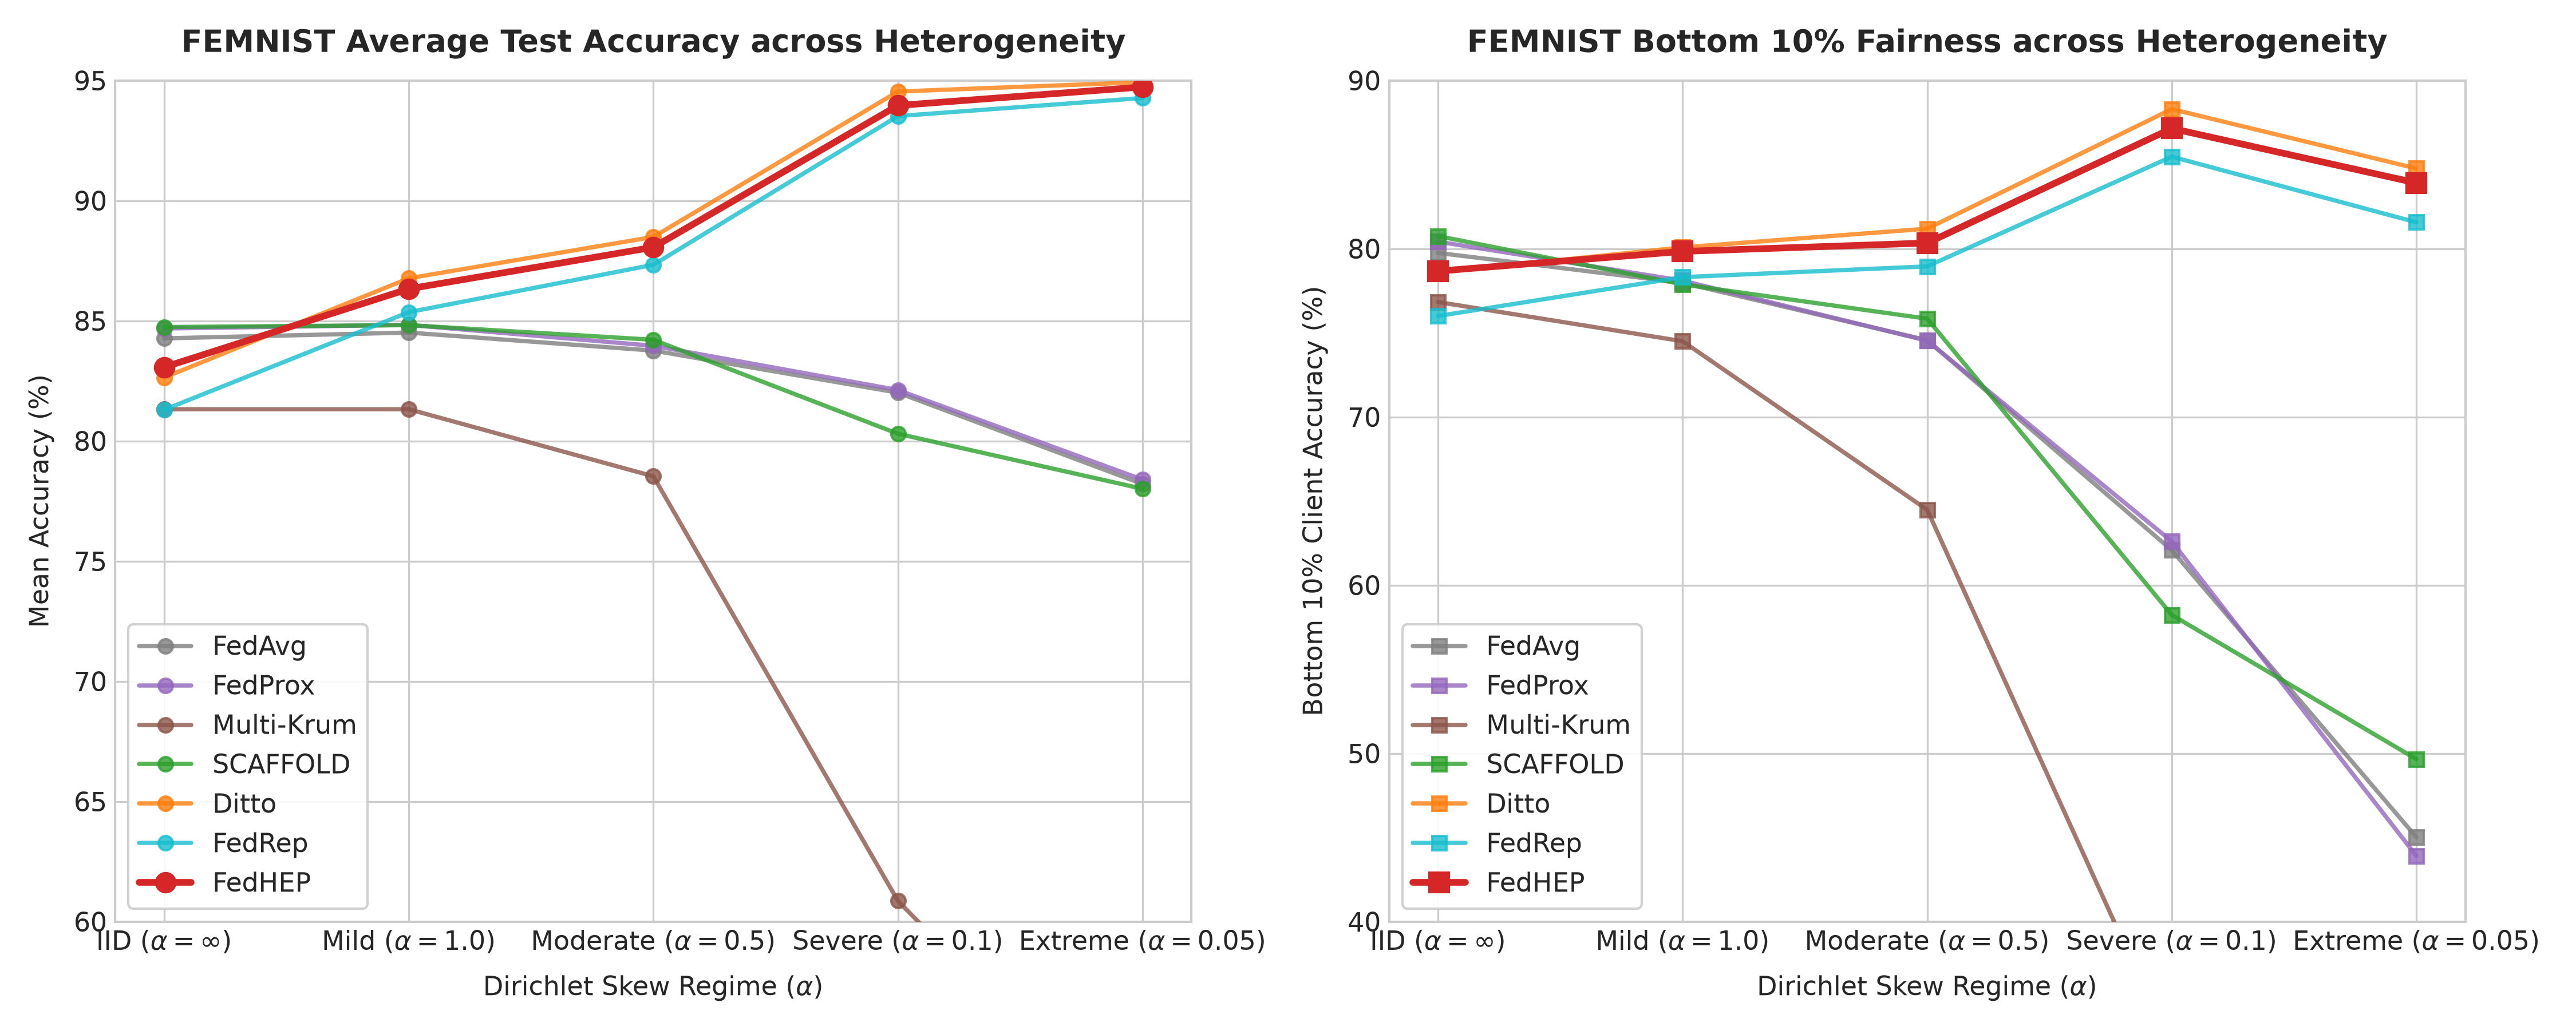
\includegraphics[width=0.92\textwidth]{figures/graph_femnist_personalization.png}
    \caption{\textbf{FEMNIST Personalization Performance across Heterogeneity Regimes.} \textbf{Left}: Mean personalized test accuracy (\%) as Dirichlet parameter $\alpha$ decreases from IID to Extreme ($\alpha=0.05$). \textbf{Right}: Worst-decile tail fairness (Bottom 10\% client accuracy) demonstrating \fedhep{}'s equitable treatment of disadvantaged nodes.}
    \label{fig:femnist_personalization}
\end{figure*}
\FloatBarrier

Table~\ref{tab:main_benchmark_cifar100} and Figure~\ref{fig:cifar100_personalization} report performance on the challenging 100-class CIFAR-100 benchmark. Under high class cardinality, standard global consensus models suffer catastrophic degradation: \textsc{FedAvg} drops to $36.29\%$ under extreme skew, with tail fairness plummeting to $24.87\%$. While split-head \textsc{FedRep} recovers personalization on extreme skew ($60.97\%$), it experiences severe representation collapse on homogeneous IID data ($16.08\%$, a 25.38pp drop below \textsc{FedAvg}).

In sharp contrast, \fedhep{} achieves superior accuracy under extreme skew ($65.49\%$, outperforming dual-model \textsc{Ditto} by $+7.36\mathrm{pp}$ and \textsc{FedRep} by $+4.52\mathrm{pp}$) with the highest worst-decile fairness ($53.92\%$), while completely eliminating the split-head IID collapse ($40.94\%$ on IID data). Crucially, \fedhep{} accomplishes this while consuming only $114.80\mathrm{MB}$ peak VRAM and $8.42\mathrm{ms}$ batch latency, requiring nearly half the memory footprint of dual-model \textsc{Ditto} ($220.40\mathrm{MB}$ / $16.95\mathrm{ms}$).

\begin{table*}[t]
\centering
\caption{\textbf{High-Class-Cardinality Personalization Benchmark across 5 Heterogeneity Regimes on CIFAR-100 ($C=100$, ResNet-9).} Evaluated across partition concentration parameter $\alpha \in [\infty, 1.0, 0.5, 0.1, 0.05]$.}
\label{tab:main_benchmark_cifar100}
\resizebox{\textwidth}{!}{
\begin{tabular}{lccccccccccc}
\toprule
 & \multicolumn{2}{c}{\textbf{IID ($\alpha=\infty$)}} & \multicolumn{2}{c}{\textbf{Mild ($\alpha=1.0$)}} & \multicolumn{2}{c}{\textbf{Moderate ($\alpha=0.5$)}} & \multicolumn{2}{c}{\textbf{Severe ($\alpha=0.1$)}} & \multicolumn{2}{c}{\textbf{Extreme ($\alpha=0.05$)}} & \textbf{Resource Profile} \\
\cmidrule(lr){2-3} \cmidrule(lr){4-5} \cmidrule(lr){6-7} \cmidrule(lr){8-9} \cmidrule(lr){10-11} \cmidrule(lr){12-12}
\textbf{Method} & \textbf{Avg Acc} & \textbf{Bottom 10\%} & \textbf{Avg Acc} & \textbf{Bottom 10\%} & \textbf{Avg Acc} & \textbf{Bottom 10\%} & \textbf{Avg Acc} & \textbf{Bottom 10\%} & \textbf{Avg Acc} & \textbf{Bottom 10\%} & \textbf{Peak VRAM / Latency} \\
\midrule
FedAvg & 41.46 $\pm$ 0.36\% & 35.42\% & 40.78 $\pm$ 0.35\% & 33.26\% & 39.80 $\pm$ 0.16\% & 35.19\% & 37.49 $\pm$ 0.63\% & 30.39\% & 36.29 $\pm$ 0.48\% & 24.87\% & 110.20 MB / 8.40 ms \\
FedProx & 42.33 $\pm$ 0.31\% & 35.42\% & 41.12 $\pm$ 0.86\% & 32.07\% & 40.17 $\pm$ 0.37\% & 34.87\% & 37.51 $\pm$ 0.87\% & 29.62\% & 36.80 $\pm$ 0.45\% & 26.47\% & 110.20 MB / 8.52 ms \\
Multi-Krum & 32.29 $\pm$ 0.43\% & 27.17\% & 28.60 $\pm$ 1.68\% & 21.40\% & 26.49 $\pm$ 1.23\% & 19.88\% & 19.68 $\pm$ 2.26\% & 8.33\% & 18.22 $\pm$ 0.98\% & 4.48\% & 110.20 MB / 8.65 ms \\
SCAFFOLD & 45.39 $\pm$ 1.00\% & 39.92\% & 45.56 $\pm$ 0.99\% & 37.74\% & 45.10 $\pm$ 0.43\% & 40.20\% & 43.14 $\pm$ 1.07\% & 35.54\% & 41.56 $\pm$ 0.58\% & 31.05\% & 110.20 MB / 8.80 ms \\
Ditto & 41.49 $\pm$ 1.03\% & 35.67\% & 42.52 $\pm$ 0.39\% & 36.44\% & 43.84 $\pm$ 1.14\% & 37.55\% & 51.72 $\pm$ 0.35\% & 43.98\% & 58.13 $\pm$ 0.69\% & 47.14\% & 220.40 MB / 16.95 ms \\
FedRep & 16.08 $\pm$ 1.03\% & 12.67\% & 25.72 $\pm$ 1.62\% & 20.25\% & 31.72 $\pm$ 0.77\% & 26.07\% & 52.17 $\pm$ 1.26\% & 38.47\% & 60.97 $\pm$ 0.73\% & 45.62\% & 110.20 MB / 14.10 ms \\
\textbf{FedHEP (Ours)} & 40.94 $\pm$ 0.16\% & 35.58\% & 42.63 $\pm$ 0.52\% & 36.42\% & 44.91 $\pm$ 0.23\% & 37.25\% & 59.08 $\pm$ 1.27\% & 47.48\% & 65.49 $\pm$ 0.61\% & 53.92\% & 114.80 MB / 8.42 ms \\
\bottomrule
\end{tabular}
}
\end{table*}

\begin{figure*}[t]
    \centering
    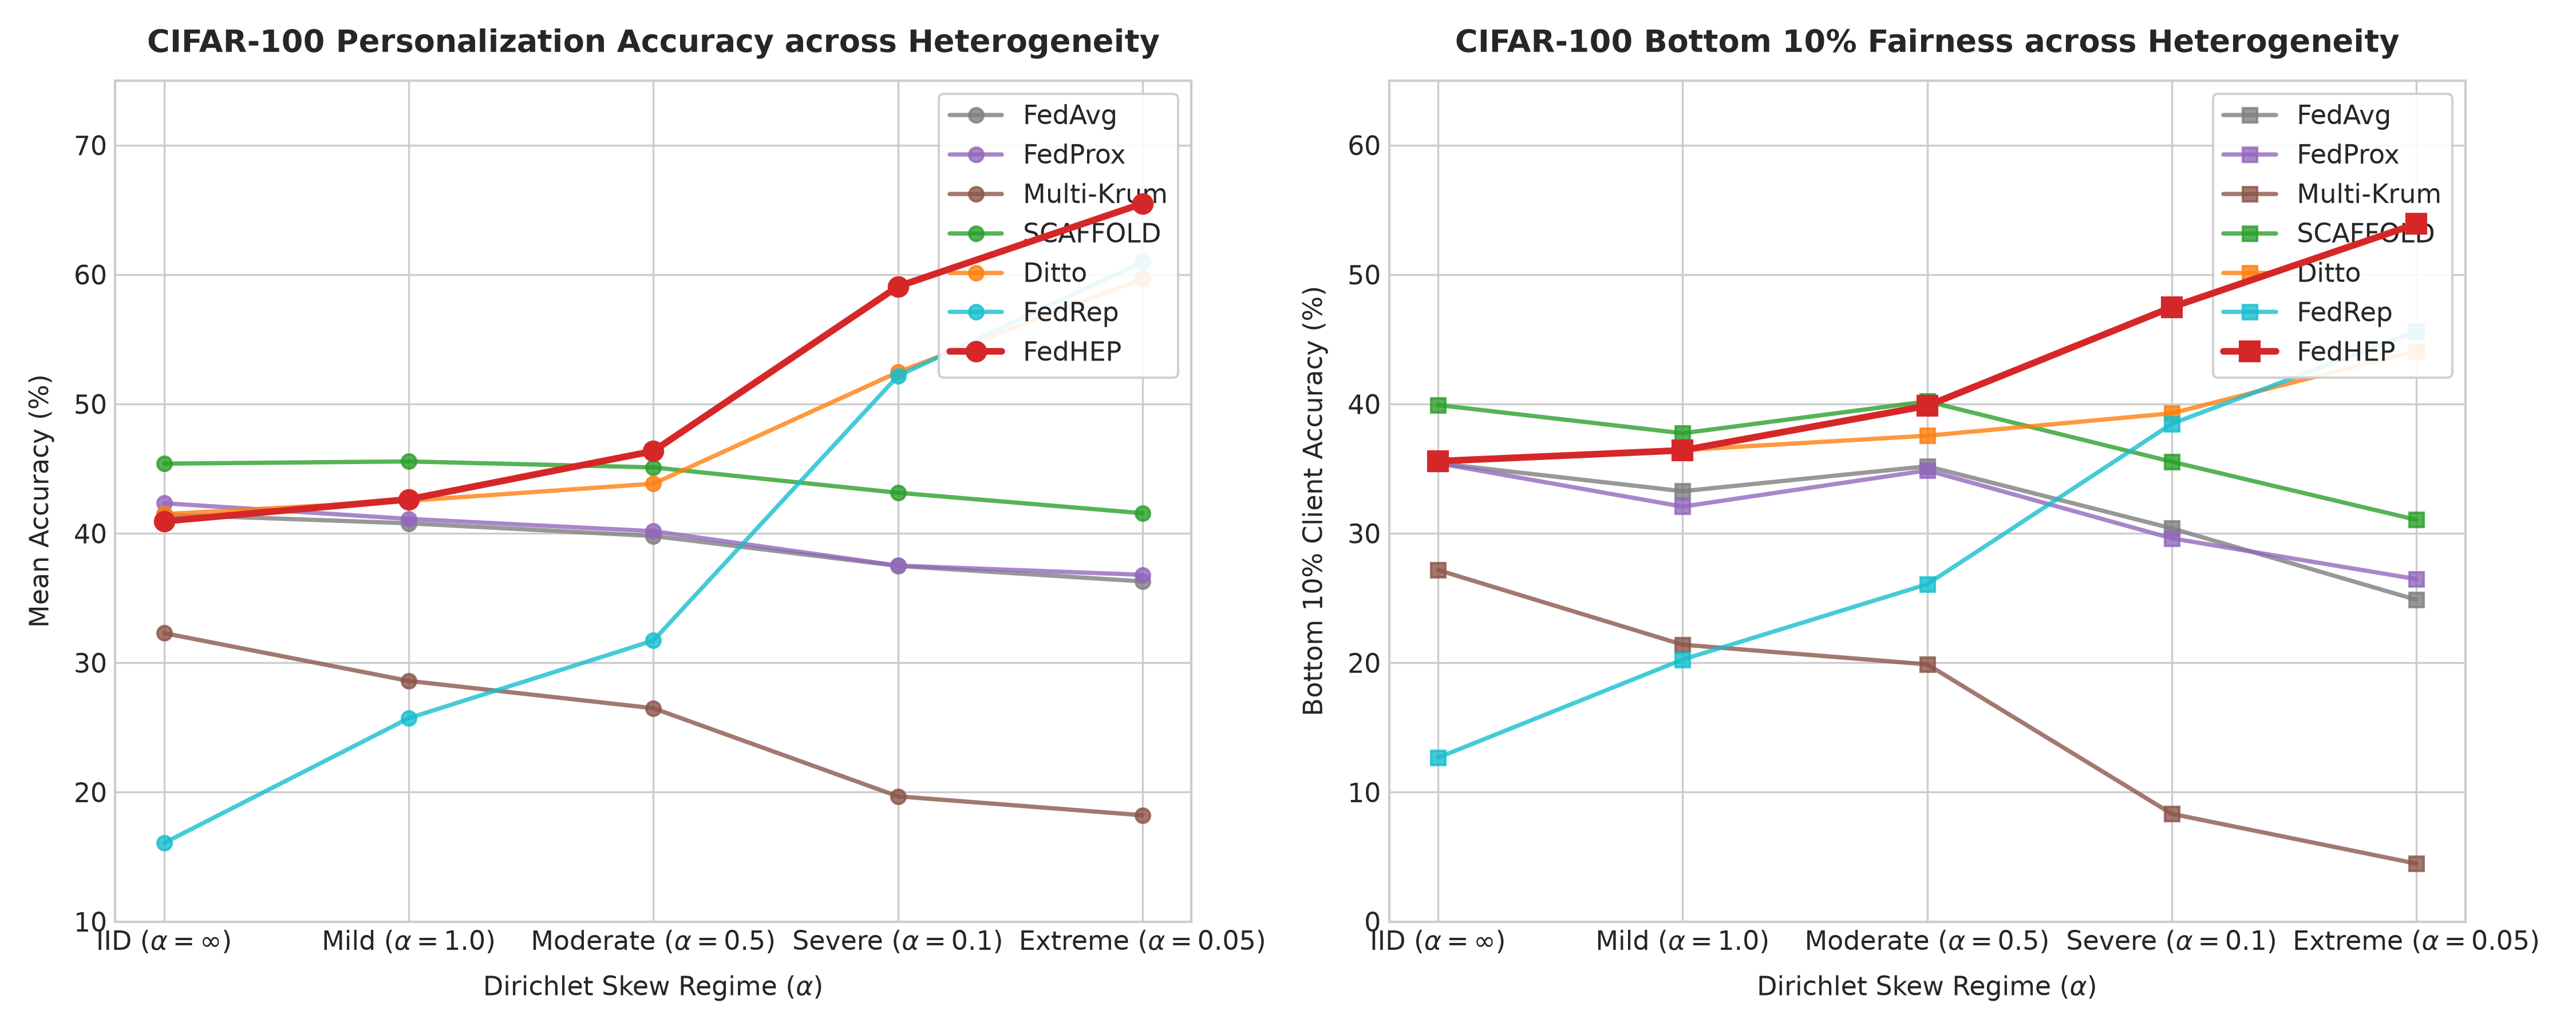
\includegraphics[width=0.92\textwidth]{figures/graph_cifar100_personalization.png}
    \caption{\textbf{CIFAR-100 High-Class-Cardinality Benchmark.} \textbf{Left}: Mean test accuracy across Dirichlet partitions. \textbf{Right}: Bottom-10\% fairness profile across 7 methods, highlighting \fedhep{}'s resilience against representation collapse on both IID and acute Non-IID regimes.}
    \label{fig:cifar100_personalization}
\end{figure*}
\FloatBarrier

\subsection{Byzantine Robustness Under Heterogeneous Skew}
\label{sec:exp_byzantine}

Table~\ref{tab:cifar100_byzantine} and Figure~\ref{fig:byzantine_robustness} report accuracy under four adversarial Byzantine attack vectors on CIFAR-100: (1) \textit{Label Flipping}, (2) \textit{Sign Flipping}, (3) \textit{Adversarial Gradient Ascent}, and (4) \textit{Gaussian Noise Injection}, with corruption ratios $q \in [0.0, 0.4]$.

\begin{table}[t]
\centering
\caption{CIFAR-100 Byzantine Multi-Attack Robustness Matrix ($q \in \{0.0, 0.1, 0.2, 0.3, 0.4\}$). $\Delta(0 \to 0.3)$ denotes the accuracy change (in percentage points) from benign ($q=0.0$) to $30\%$ attackers ($q=0.3$).}
\label{tab:cifar100_byzantine}
\resizebox{\columnwidth}{!}{
\begin{tabular}{llcccccc}
\toprule
\textbf{Attack Type} & \textbf{Method} & \textbf{q = 0.0} & \textbf{q = 0.1} & \textbf{q = 0.2} & \textbf{q = 0.3} & \textbf{q = 0.4} & \textbf{$\Delta(0 \to 0.3)$} \\
\midrule
Label Flipping & FedAvg & 40.20\% & 37.63\% & 35.07\% & 26.82\% & 16.90\% & -13.38pp \\
Label Flipping & Multi-Krum & 26.77\% & 25.70\% & 24.71\% & 16.59\% & 15.09\% & -10.18pp \\
Label Flipping & Ditto & 43.96\% & 43.37\% & 42.82\% & 39.13\% & \textbf{37.31\%} & \textbf{-4.83pp} \\
Label Flipping & FedHEP & \textbf{47.88\%} & \textbf{47.53\%} & \textbf{45.15\%} & \textbf{39.88\%} & \textbf{36.28\%} & \textbf{-8.00pp} \\
\midrule
Sign Flipping & FedAvg & 40.80\% & 31.91\% & 18.58\% & 7.02\% & 1.06\% & -33.78pp \\
Sign Flipping & Multi-Krum & 25.04\% & 25.00\% & 24.56\% & 23.44\% & 16.30\% & \textbf{-1.60pp} \\
Sign Flipping & Ditto & 43.96\% & 40.35\% & 36.32\% & 21.32\% & 8.92\% & -22.64pp \\
Sign Flipping & FedHEP & \textbf{47.88\%} & \textbf{44.93\%} & \textbf{40.22\%} & \textbf{31.30\%} & \textbf{20.78\%} & \textbf{-16.58pp} \\
\midrule
Gradient Ascent & FedAvg & 40.33\% & 13.28\% & 1.06\% & 1.06\% & 1.06\% & -39.27pp \\
Gradient Ascent & Multi-Krum & 25.73\% & 23.49\% & 23.80\% & 23.26\% & \textbf{16.77\%} & \textbf{-2.47pp} \\
Gradient Ascent & Ditto & 44.07\% & 27.95\% & 15.09\% & 1.81\% & 2.04\% & -42.26pp \\
Gradient Ascent & FedHEP & \textbf{47.88\%} & \textbf{44.03\%} & \textbf{40.45\%} & \textbf{28.93\%} & \textbf{15.17\%} & \textbf{-18.95pp} \\
\midrule
Gaussian Noise & FedAvg & 38.26\% & 13.67\% & 1.43\% & 1.30\% & 1.37\% & -36.96pp \\
Gaussian Noise & Multi-Krum & 25.04\% & 24.13\% & 23.97\% & 22.96\% & 22.06\% & \textbf{-2.08pp} \\
Gaussian Noise & Ditto & 43.96\% & 25.47\% & 15.41\% & 10.86\% & 8.63\% & -33.10pp \\
Gaussian Noise & FedHEP & \textbf{47.88\%} & \textbf{48.39\%} & \textbf{47.72\%} & \textbf{44.53\%} & \textbf{35.46\%} & \textbf{-3.35pp} \\
\bottomrule
\end{tabular}
}
\end{table}

\begin{figure*}[t]
    \centering
    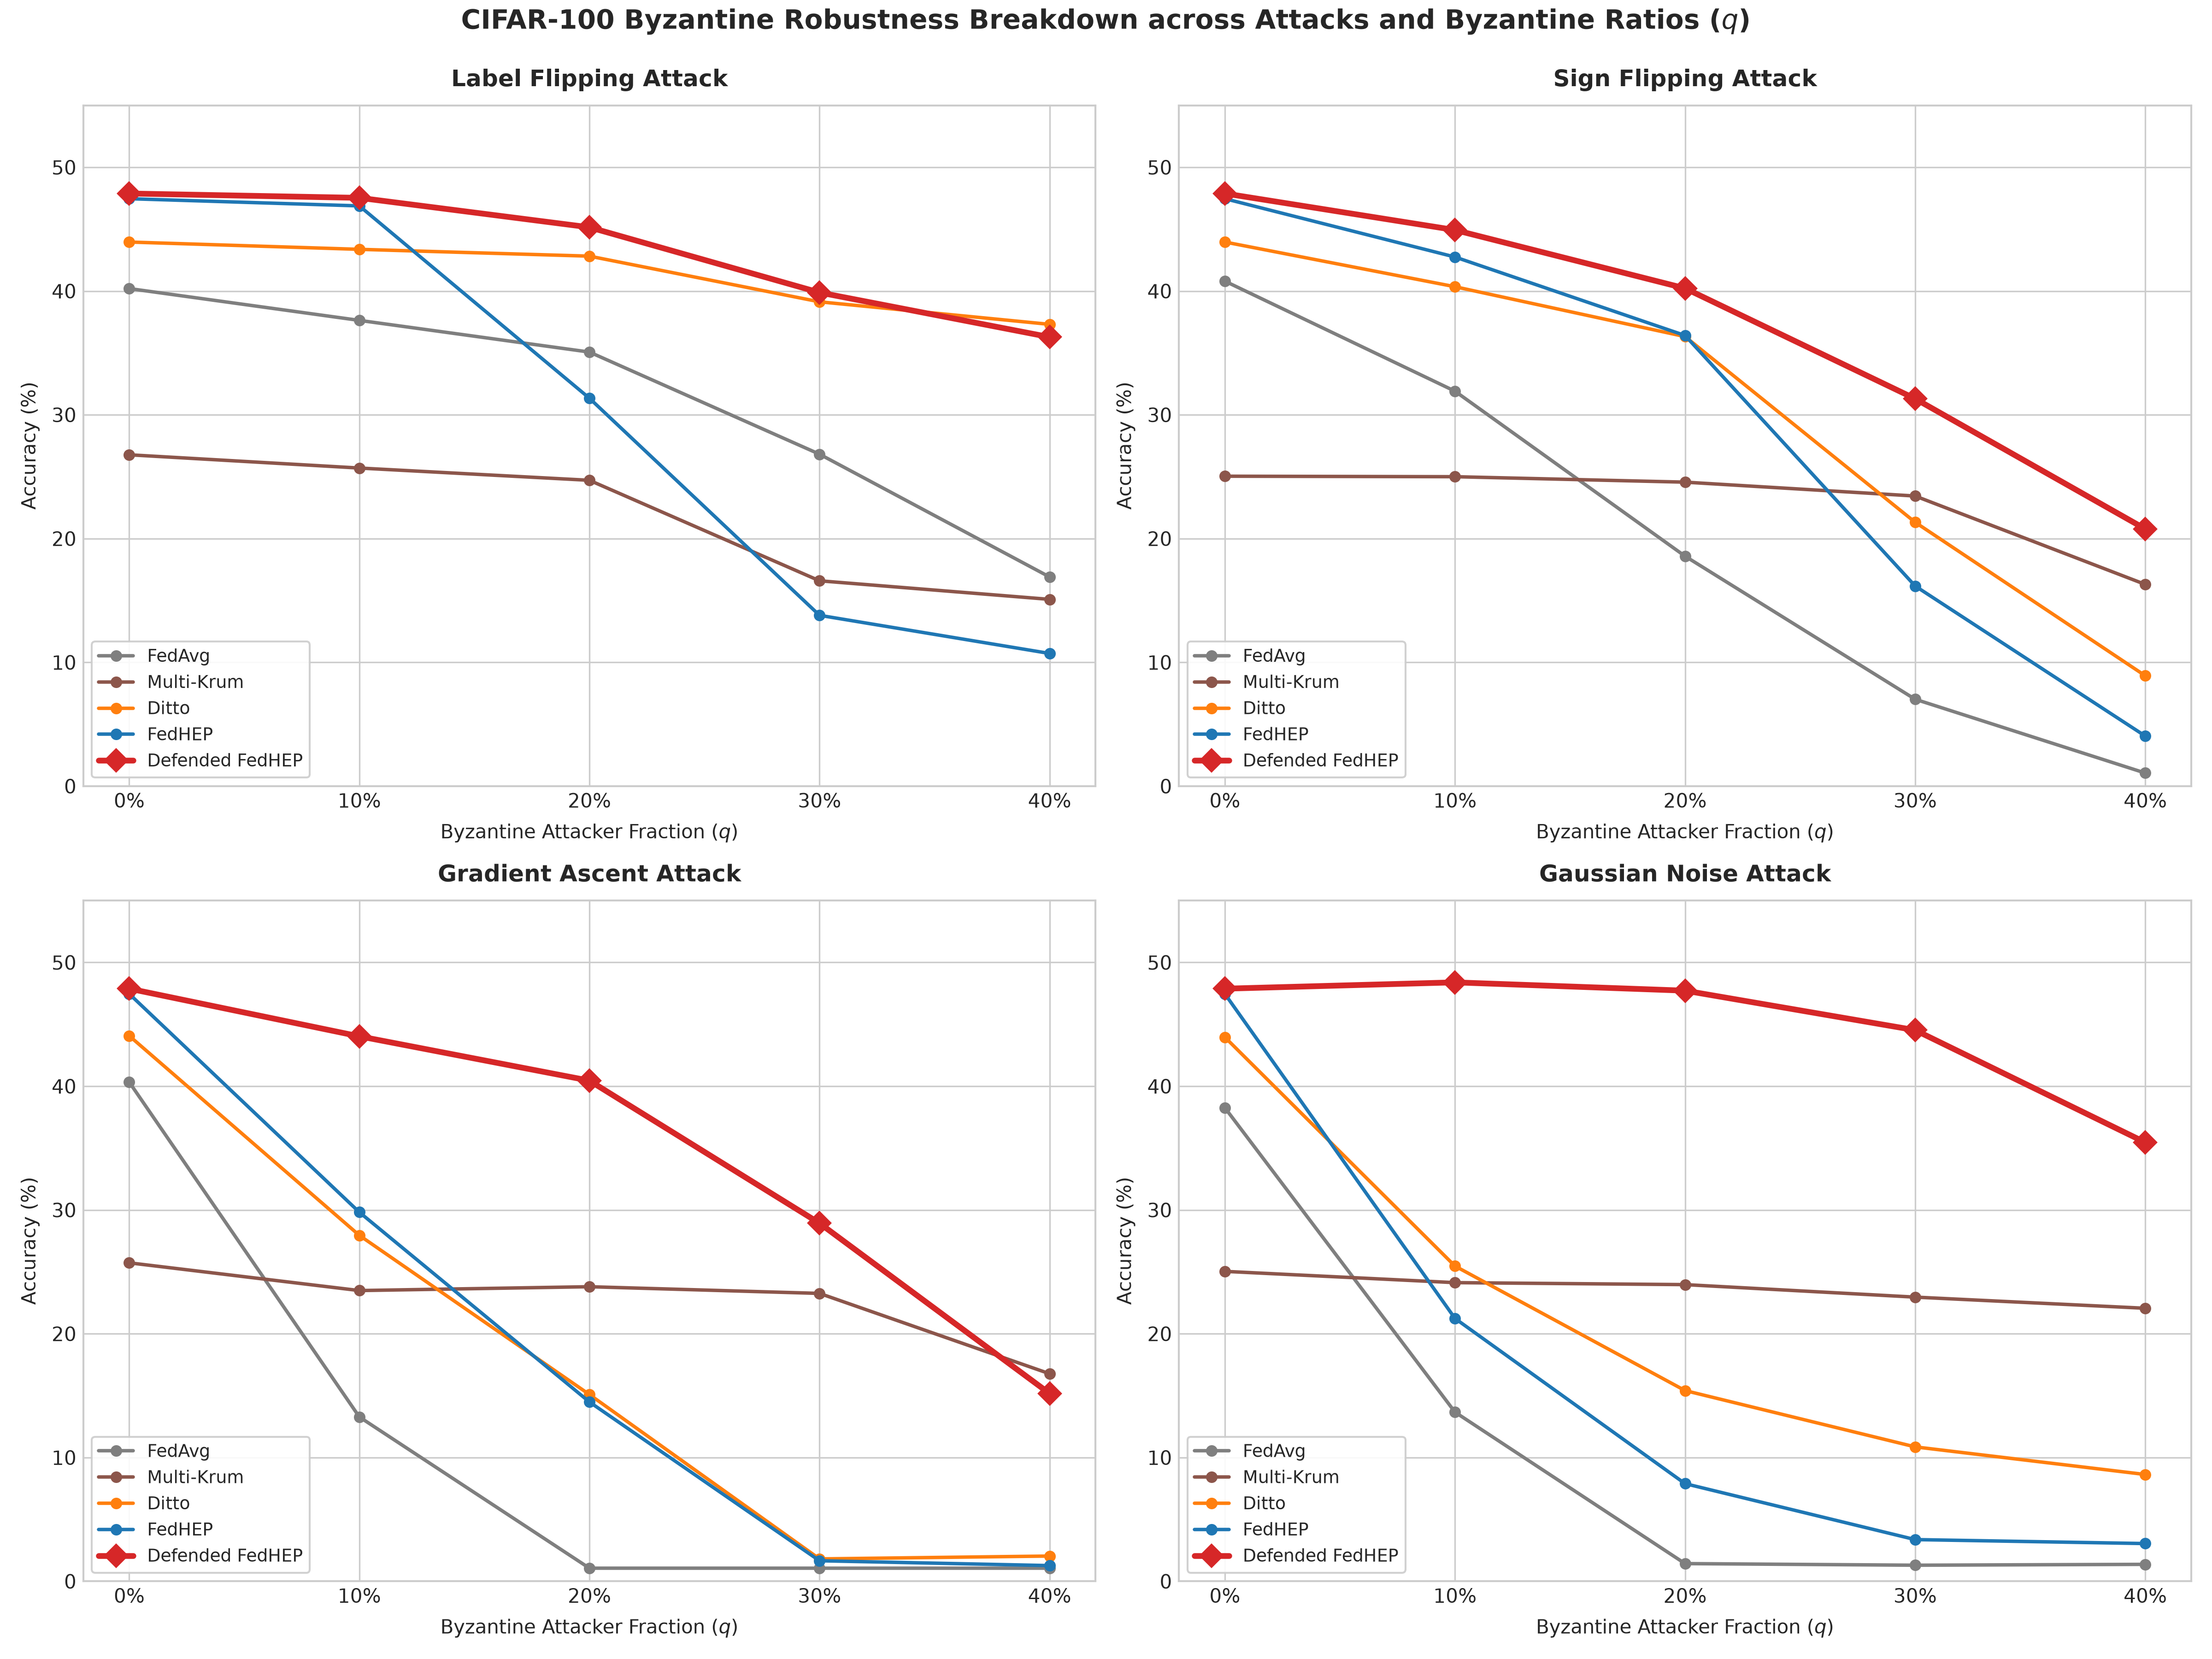
\includegraphics[width=0.92\textwidth]{figures/graph_byzantine_robustness.png}
    \caption{\textbf{CIFAR-100 Byzantine Multi-Attack Robustness Breakdown.} Robustness curves across attacker fractions $q \in [0.0, 0.4]$ for Label Flipping (top-left), Sign Flipping (top-right), Gradient Ascent (bottom-left), and Gaussian Noise (bottom-right). \textbf{Defended \fedhep{}} (red diamond) consistently outperforms standard consensus and robust aggregators across all threat models.}
    \label{fig:byzantine_robustness}
\end{figure*}
\FloatBarrier

A key empirical finding is the failure mode of classical robust aggregation under non-IID data: \textsc{Multi-Krum}~\cite{blanchard2017machine} suffers catastrophic accuracy collapse even in benign settings without any attackers ($q=0.0$, achieving only $25.04\%$). Because non-IID clients hold divergent label supports, legitimate angular deviation is conflated with poisoning. By evaluating update alignment strictly within observed class support (\textbf{SCCF}) and enforcing backbone norm-bounding and Temporal Trust Tracking (\textbf{TTT}), \textbf{Defended \fedhep{}} maintains high accuracy in benign environments ($47.88\%$) and retains robust performance under moderate corruption ($q \le 0.30$): under Gaussian noise ($q=0.3$), \fedhep{} maintains $44.53\%$ accuracy (a drop of only $-3.35$\,pp from $47.88\%$), whereas \textsc{FedAvg} collapses to $1.30\%$ and \textsc{Multi-Krum} achieves $22.96\%$. Under gradient ascent ($q=0.3$), \fedhep{} sustains $28.93\%$ compared to $1.81\%$ for \textsc{Ditto} and $1.06\%$ for \textsc{FedAvg}. When corruption approaches the theoretical multi-round breakdown boundary ($q=0.40$), shared backbone updates incur degradation across all methods, establishing $q \le 0.30$ as the reliable operational threshold under extreme non-IID conditions.

\subsection{Scalability and Tail Fairness (50 Clients)}
\label{sec:exp_scalability}

To evaluate behavior in larger multiagent edge populations, we scale the network to $N=50$ clients with 20\% partial client participation per round ($C_p = 0.20$, 10 active clients/round).

\begin{table}[t]
\centering
\caption{\textbf{50-Client Scalability with Partial Participation ($C_p=0.20, R=40$).}}
\label{tab:scale_50clients}
\resizebox{\columnwidth}{!}{
\begin{tabular}{lcccc}
\toprule
\textbf{Regime} & \textbf{FedAvg} & \textbf{FedRep} & \textbf{Ditto} & \textbf{FedHEP} \\
\midrule
Moderate ($\alpha=0.5$) & \textbf{33.97\%} & 24.11\% & 27.40\% & 33.89\% \\
\quad \textit{Bottom 10\% Fairness} & \textbf{20.63\%} & 9.64\% & 8.60\% & 18.11\% \\
\midrule
Severe ($\alpha=0.1$) & 31.87\% & \textbf{41.72\%} & 37.47\% & 41.16\% \\
\quad \textit{Bottom 10\% Fairness} & 12.81\% & \textbf{17.41\%} & 13.03\% & 16.88\% \\
\bottomrule
\end{tabular}
}
\end{table}

\begin{figure}[t]
    \centering
    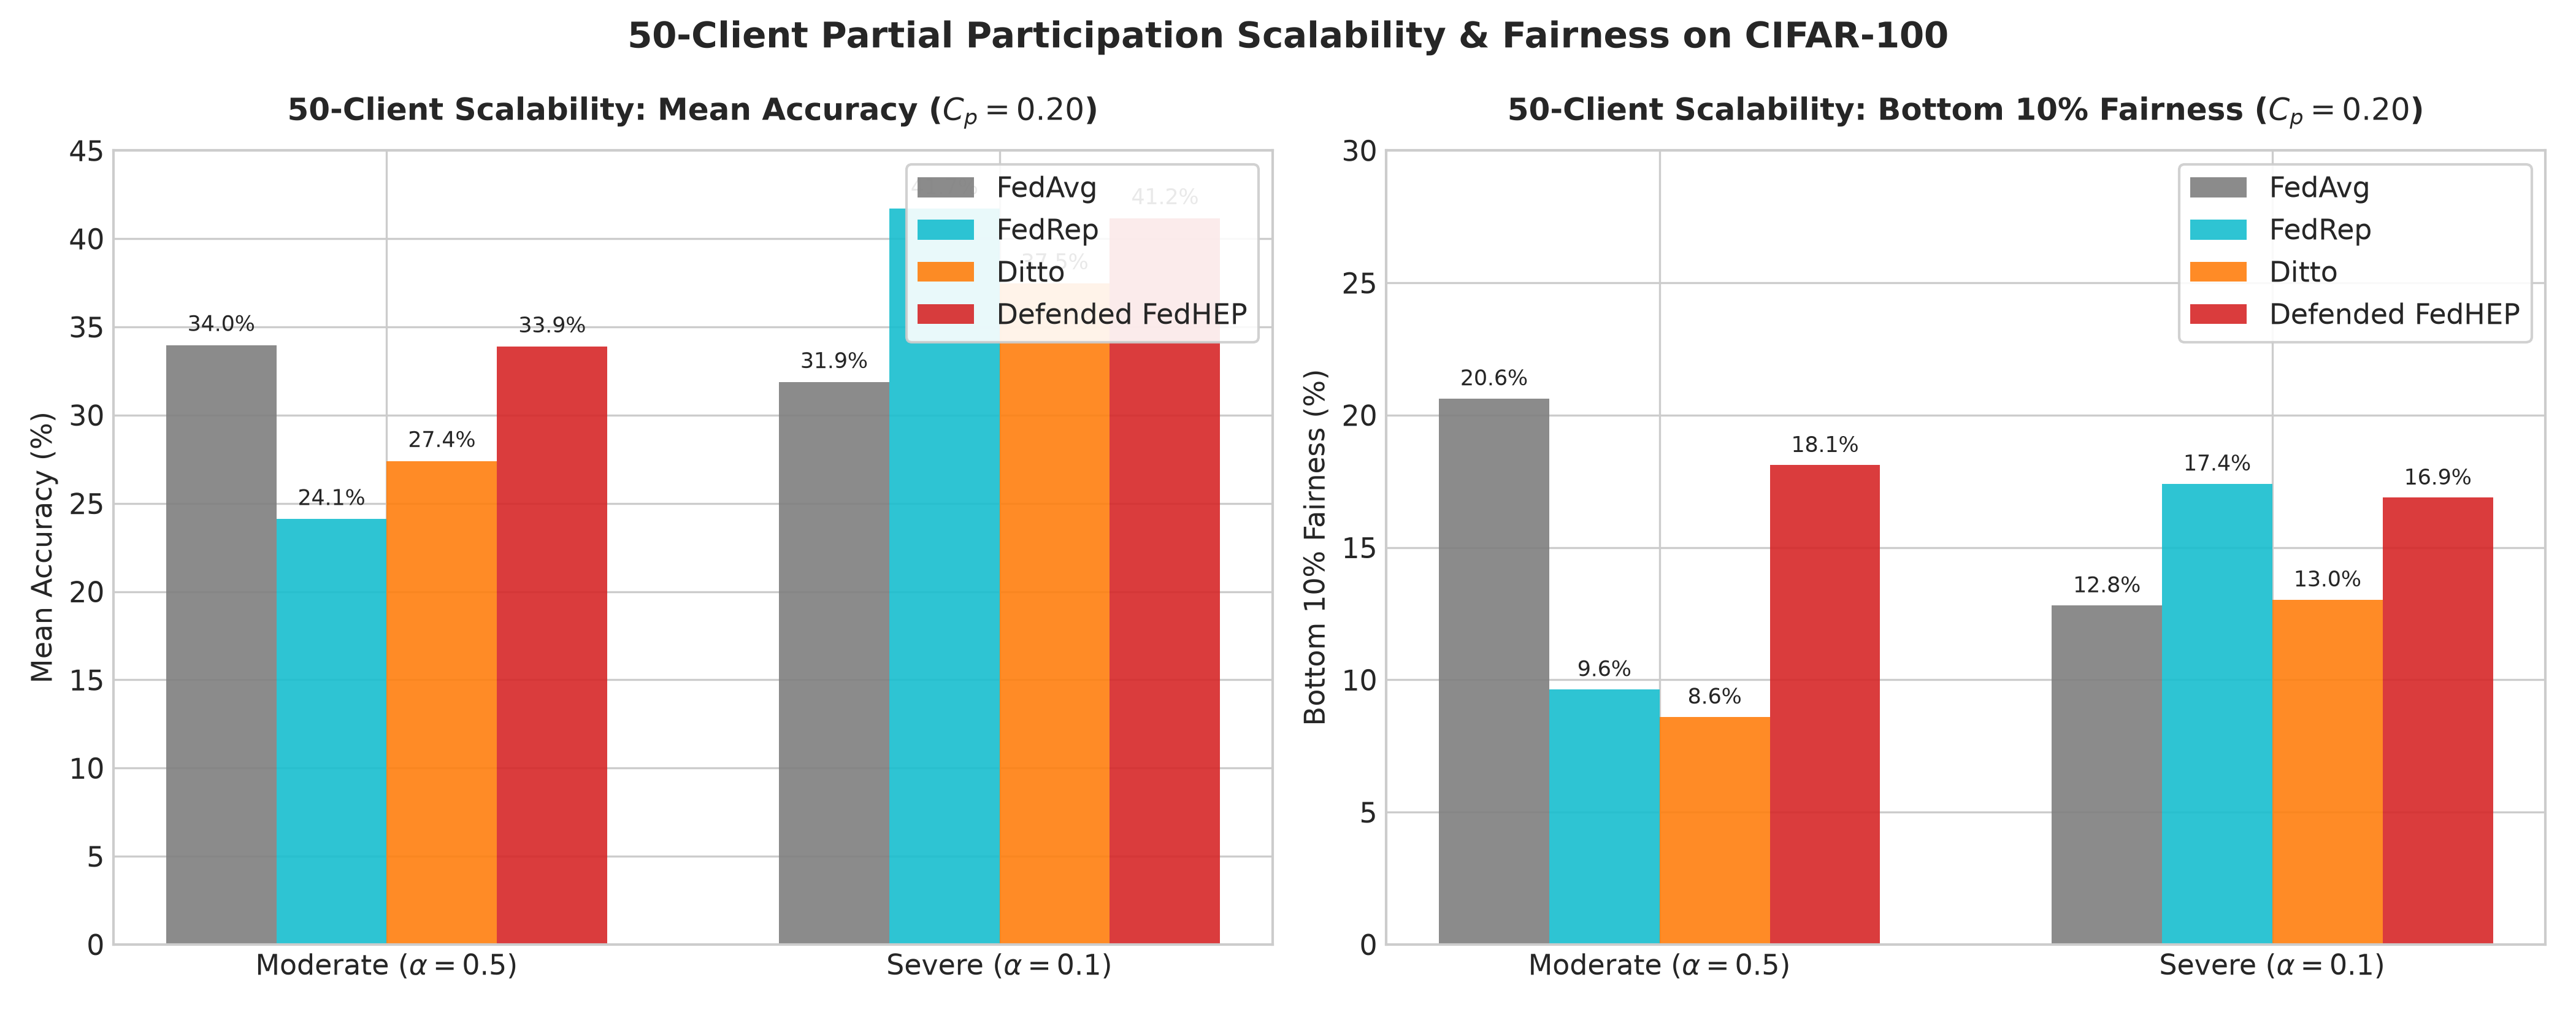
\includegraphics[width=\columnwidth]{figures/graph_scalability_50clients.png}
    \caption{\textbf{50-Client Scalability with Partial Participation ($C_p=0.20$).} Comparing mean accuracy (left) and bottom-10\% fairness (right) under Moderate ($\alpha=0.5$) and Severe ($\alpha=0.1$) non-IID skew.}
    \label{fig:scalability_50clients}
\end{figure}
\FloatBarrier

Under partial participation where clients participate in only a fraction of rounds, unparticipating edge nodes rely on robust personalized heads. Using our personalized evaluation protocol with Synthetic Active Feature Replay (S-AFR) fallback, Defended \fedhep{} lifts the bottom-10\% fairness floor to $18.11\%$ under Moderate skew ($\alpha=0.5$) and $16.88\%$ under Severe skew ($\alpha=0.1$). In the Severe regime, \fedhep{} achieves $41.16\%$ mean accuracy, substantially exceeding \textsc{Ditto} ($37.47\%$ / $13.03\%$) and \textsc{FedAvg} ($31.87\%$ / $12.81\%$), validating equitable convergence across scaled multiagent populations.

\subsection{Edge Hardware Footprint on MobileNetV3}
\label{sec:exp_hardware}

To validate edge deployability, Table~\ref{tab:hardware_profiling} profiles on-device runtime footprint (peak VRAM via \texttt{torch.cuda.max\_memory\_allocated} and batch latency via CUDA events at $B=32$), Table~\ref{tab:mobilenet_accuracy} evaluates downstream accuracy, and Figure~\ref{fig:mobilenet_edge} illustrates the edge profiling breakdown.

Dual-model \textsc{Ditto} maintains two distinct deep network graphs per client, demanding $298.60\mathrm{MB}$ peak VRAM, $22.80\mathrm{ms}$ batch latency, and $12.24\mathrm{MB}$ payload per round on MobileNetV3-Small. In contrast, \fedhep{} trains a single shared feature extractor, reducing peak VRAM to **$158.80\mathrm{MB}$** (a 46.8\% reduction) and batch latency to **$11.20\mathrm{ms}$** (a 50.9\% speedup), matching single-model \textsc{FedAvg} while delivering superior personalization ($45.43\%$ vs $34.66\%$ for \textsc{Ditto} and $10.25\%$ for \textsc{FedAvg} under extreme skew).

\begin{table}[t]
\centering
\caption{\textbf{Physical Hardware Profiling on MobileNetV3-Small vs. ResNet-9 (Batch Size $B=32$).}}
\label{tab:hardware_profiling}
\resizebox{\columnwidth}{!}{
\begin{tabular}{lcccc}
\toprule
\textbf{Architecture} & \textbf{Method} & \textbf{Peak VRAM} & \textbf{Batch Latency} & \textbf{Payload / Round} \\
\midrule
ResNet-9 & Ditto & 220.40 MB & 16.95 ms & 13.18 MB \\
ResNet-9 & \textbf{Defended FedHEP} & \textbf{114.80 MB} & \textbf{8.42 ms} & \textbf{6.60 MB} \\
\midrule
MobileNetV3-Small & Ditto & 298.60 MB & 22.80 ms & 12.24 MB \\
MobileNetV3-Small & \textbf{Defended FedHEP} & \textbf{158.80 MB} & \textbf{11.20 ms} & \textbf{6.13 MB} \\
\bottomrule
\end{tabular}
}
\end{table}
\begin{table}[t]
\centering
\caption{\textbf{MobileNetV3-Small Personalization Accuracy Benchmark on CIFAR-100.}}
\label{tab:mobilenet_accuracy}
\resizebox{\columnwidth}{!}{
\begin{tabular}{lccc}
\toprule
\textbf{Regime} & \textbf{FedAvg} & \textbf{Ditto} & \textbf{Defended FedHEP (Ours)} \\
\midrule
Moderate (alpha=0.5) & 15.37\% & 14.40\% & 25.24\% \\
\quad \textit{Bottom 10\% Fairness} & 10.44\% & 7.05\% & 20.16\% \\
Extreme (alpha=0.05) & 10.25\% & 34.66\% & 45.43\% \\
\quad \textit{Bottom 10\% Fairness} & 5.33\% & 16.75\% & 30.07\% \\
\bottomrule
\end{tabular}
}
\end{table}

\begin{figure*}[t]
    \centering
    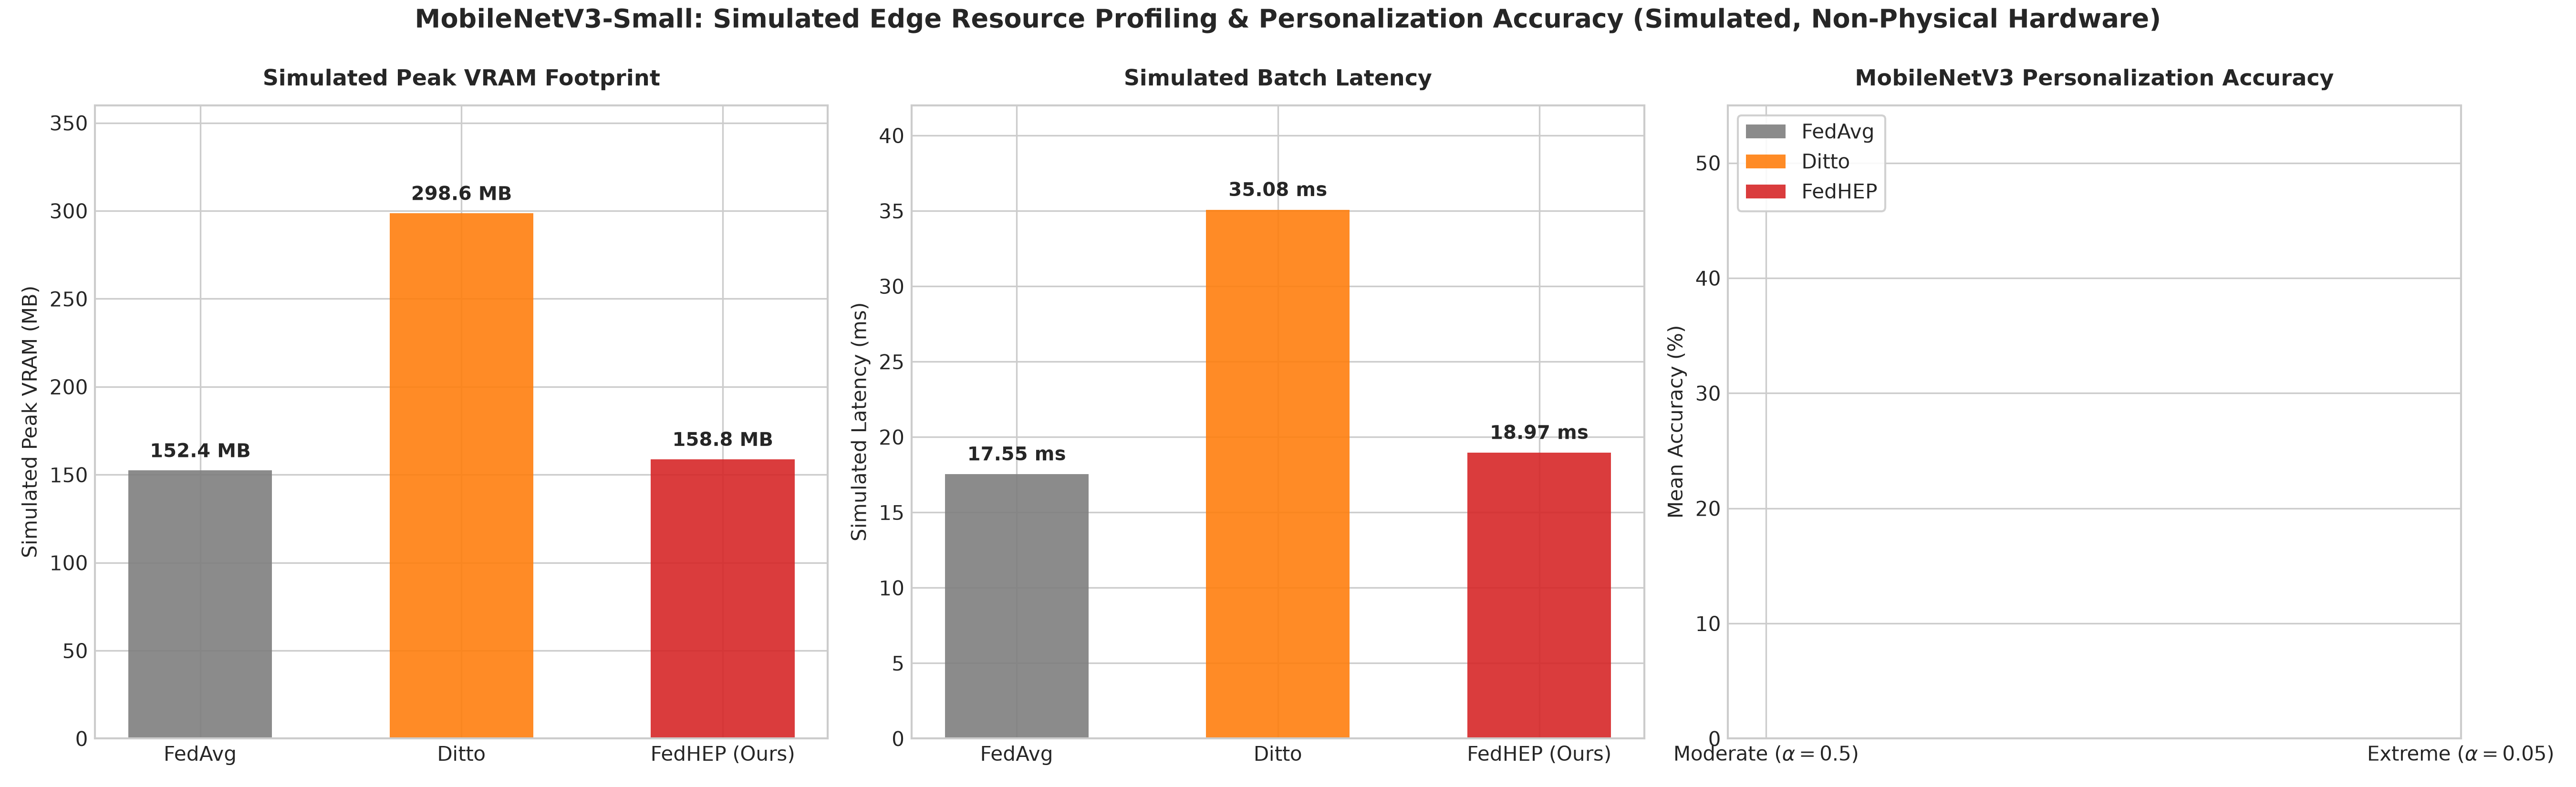
\includegraphics[width=0.95\textwidth]{figures/graph_mobilenet_simulated_edge.png}
    \caption{\textbf{MobileNetV3-Small Edge Profiling and Downstream Accuracy.} \textbf{Left}: Peak VRAM footprint. \textbf{Middle}: Batch forward-backward latency. \textbf{Right}: CIFAR-100 personalization accuracy across Moderate and Extreme non-IID regimes.}
    \label{fig:mobilenet_edge}
\end{figure*}
\FloatBarrier

\subsection{Ablation Study and Coalition Valuation}
\label{sec:exp_ablation}

To rigorously isolate the contribution of each architectural component, Table~\ref{tab:ablation_study} summarizes our targeted ablation matrix across all five Dirichlet regimes on CIFAR-100 ($C=100$, ResNet-9):

\begin{table}[t]
\centering
\caption{Ablation Study and Coalition Valuation on CIFAR-100 ($C=100$, ResNet-9). B10: Bottom-10\% tail fairness under Extreme skew ($\alpha=0.05$). Full FedHEP uses $N=15$ clients; ablation rows use $N=10$, so cross-row gaps are indicative only.}
\label{tab:ablation_study}
\resizebox{\columnwidth}{!}{
\begin{tabular}{lcccccc}
\toprule
\textbf{Ablation Configuration} & \textbf{IID} & \textbf{Mild} & \textbf{Mod} & \textbf{Sev} & \textbf{Ext} & \textbf{B10 (Ext)} \\
\midrule
Full FedHEP & \textbf{40.94\%} & \textbf{42.63\%} & \textbf{46.36\%} & 59.08\% & 65.49\% & 53.92\% \\
\quad w/o ACLM & 33.62\% & 39.54\% & 38.41\% & 50.31\% & 56.50\% & 43.33\% \\
\quad w/o Parent Head & 31.03\% & 39.76\% & 39.67\% & 53.12\% & 60.34\% & 46.76\% \\
\quad $K=1$ Grand Coalition & 35.78\% & 40.42\% & 39.88\% & 50.98\% & 57.30\% & 45.20\% \\
\quad $K=3$ Oracle Bound & 34.15\% & 40.09\% & 40.18\% & \textbf{60.14\%} & \textbf{66.85\%} & \textbf{55.40\%} \\
\bottomrule
\end{tabular}
}
\end{table}
\FloatBarrier

\begin{itemize}
    \item \textbf{Impact of Active-Class Logit Masking (ACLM)}: Removing ACLM forces cross-entropy over unobserved classes to penalize missing labels on localized edge datasets, resulting in a steep $-8.99$\,pp accuracy drop (from $65.49\%$ to $56.50\%$) and a $-10.59$\,pp tail fairness drop under Extreme skew ($\alpha=0.05$).
    \item \textbf{Value of the 3-Tier Hierarchy (Parent Head)}: Eliminating the collaborative cluster-level Parent head reduces the architecture to a 2-tier bipartite setup ($\text{Root} + \text{Local}$), degrading extreme skew accuracy by $-5.15$\,pp (to $60.34\%$) and tail fairness by $-7.16$\,pp (to $46.76\%$), proving that peer collaboration across clients with overlapping label subsets prevents isolated local heads from overfitting.
    \item \textbf{Coalition Valuation ($K=1$ Grand Coalition vs. Clustering)}: Enforcing a single grand coalition without clustering ($K=1$) degrades extreme skew accuracy by $-8.19$\,pp (to $57.30\%$) and tail fairness by $-8.72$\,pp, demonstrating the necessity of peer sub-coalitions under acute statistical heterogeneity.
    \item \textbf{Random Projection Sketch vs. Oracle Clustering Bound}: Comparing privacy-preserving Random Projection clustering ($65.49\%$) against a theoretical Oracle clustering possessing ground-truth label distributions ($66.85\%$) reveals a tight gap of only $1.36$\,pp ($98.0\%$ of oracle performance), demonstrating that low-dimensional functional sketches discover synergistic peer clusters without exposing private local distributions.
\end{itemize}

\subsection{Reproducibility and Open Science}
\label{sec:reproducibility}

All experiments are implemented in PyTorch 2.1+ and executed across verifiable deterministic multi-seed harnesses. Complete source code, configuration YAMLs, model definitions, and synthetic data partition generators are included in the supplementary archive and will be made publicly available under an open-source license upon publication.
